\documentclass[14pt,a4paper]{scrartcl}
\usepackage[utf8]{inputenc}
\usepackage[english,russian, ukrainian]{babel}
\usepackage{misccorr, color, ragged2e, amsfonts, amsthm, graphicx, systeme, amsmath, mdframed, lipsum, setspace, mathtools, esint, color, listings}

\renewcommand\qedsymbol{$\blacksquare$}
\renewcommand*{\proofname}{\text{Доведення}}

\theoremstyle{definition}
\newtheorem*{defo}{Означення}
\newtheorem*{teo}{Теорема}
\newtheorem*{example}{Приклад}
\theoremstyle{remark}
\newtheorem*{remark}{Зауваження}
\theoremstyle{definition}
\newtheorem*{consequence}{Наслідок}
\theoremstyle{definition}
\newtheorem{statement}{Утверждение}[section]
\newmdtheoremenv{boxteo}{Теорема}[section]
\newtheorem{look}{Позначення}[section]

\setlength\parindent{0pt}

\DeclareMathOperator*\lowlim{\underline{lim}}
\DeclareMathOperator*\uplim{\overline{lim}}

\newcommand\independent{\protect\mathpalette{\protect\independenT}{\perp}}

\def\independenT#1#2{\mathrel{\rlap{$#1#2$}\mkern2mu{#1#2}}}

% Default fixed font does not support bold face
\DeclareFixedFont{\ttb}{T1}{txtt}{bx}{n}{12} % for bold
\DeclareFixedFont{\ttm}{T1}{txtt}{m}{n}{12}  % for normal

\definecolor{deepblue}{rgb}{0,0,0.5}
\definecolor{deepred}{rgb}{0.6,0,0}
\definecolor{deepgreen}{rgb}{0,0.5,0}

\doublespacing

\begin{document}

\def\be{\begin{equation}}
\def\ee{\end{equation}}

\def\bd{\begin{defo}}
\def\ed{\end{defo}}

\def\bbt{\begin{boxteo}}
\def\ebt{\end{boxteo}}

\def\i{\infty}
\def\d{\partial}

\begin{titlepage}
\begin{center}

\vspace*{0.1cm}
\vfill

{\huge \textbf{ТЕОРІЯ СТІЙКОСТІ}}\\
\vspace{5cm}
За лекціями Горбань Н.\\
\vspace{1cm}
Редактори: Терещенко Д.\\ \hspace{3.7cm} Людомирський Ю.

\vfill

2021

\end{center}
\end{titlepage}


\tableofcontents
\newpage

\section{Лекція 1}
\subsection{Нормальні системи диференційних рівнянь}


\be
\left\lbrace
\begin{gathered}
x'_1 (t) = f_1(t, x_1 (t), ... , x_n(t)) \\
x'_2 (t) = f_2(t, x_1 (t), ... , x_n(t)) \\
\vdots \\
    x'_n (t) = f_n(t, x_1 (t), ... , x_n(t)) \\
\end{gathered}\right.
\ee

 Системою диф. рівнянь n-го порядку в нормальній формі називається система вигляду (1), де $ f_i : D \to \mathbb{R}, \quad D \subset \mathbb{R}^{n+1 }, \quad i = \overline{1, n}$.
\look
\[
      \overline{x}(t) = \left(\begin{array}{l}
      x_1(t)    \\
      \dots     \\
      x_n(t)
      \end{array}\right) \text{-- невідома вектор-функція}, \quad
      \overline{f}(t, \overline{x}(t)) = \left(\begin{array}{l}
      f_1     \\
      \dots  \\
      f_n
      \end{array}\right) \text{, що}
\]
$D \rightarrow \mathbb{R}, \quad D \subset \mathbb{R}^{n+1}$, тоді $(1): \overline{x}'(t) = \overline{f}(t, \overline{x}(t))$.


\def\rect{\textbf{П}}
\bd
\textbf{Розв'язком системи} (1) на $(\alpha , \beta)$ називається така вектор-функція $\overline{x} (t) \in C(\alpha , \beta)$, що:
\begin{enumerate}
  \item $(t, x_1(t), \dots, x_n(t)) \in D \quad \forall t \in (\alpha, \beta)$;
  \item $\overline{x}(t)$  перетворює $(1)$ на тотожність на інтервалі $(\alpha, \beta)$.
\end{enumerate}

\textbf{Загальним розв'язком системи}  (1) називається n-параметрична сім'я розв'язків (1), що охоплює всі розв'язки системи.
\ed

Задача Коші. Для заданих $t_0, \overline{x}^{0} \in D$ знайти такий розв'язок (1), що $\overline{x} (t_0) = \overline{x}^{0}$.

\begin{boxteo}[Теорема Пеано]
Нехай $\Pi = \{(t, \overline{x}) \in \mathbb{R} \quad \big| \quad |t-t_0| \leq a, \quad ||\overline{x} - \overline{x}_0|| \leq b \}$ та $\overline{f} \in C(\Pi)$. Тоді розв'язок задачі Коші:
\begin{gather*}
  \begin{cases}
    \overline{x}' = \overline{f}(t, \overline{x}) \\
    \overline{x}(t_0) = \overline{x}_0
  \end{cases}
\end{gather*}
існує принаймні на проміжку $I_h = (t_0 - h, t_0 + h)$, де $h = \min\{{a, \dfrac{b}{M}}\}$, \\ $M = \max\limits_{(t, x) \in \Pi} {||\overline{f}(t, \overline{x})||}$.
\end{boxteo}

\begin{boxteo}[про продовження]
    Нехай $\overline{f} \in \mathbb{C}(D), D \subset \mathbb{R}^{n+1}$ - деяка обмежена область. Нехай $(t_0, \overline{x}^0) \in D$ - задана точка.

    \begin{center} 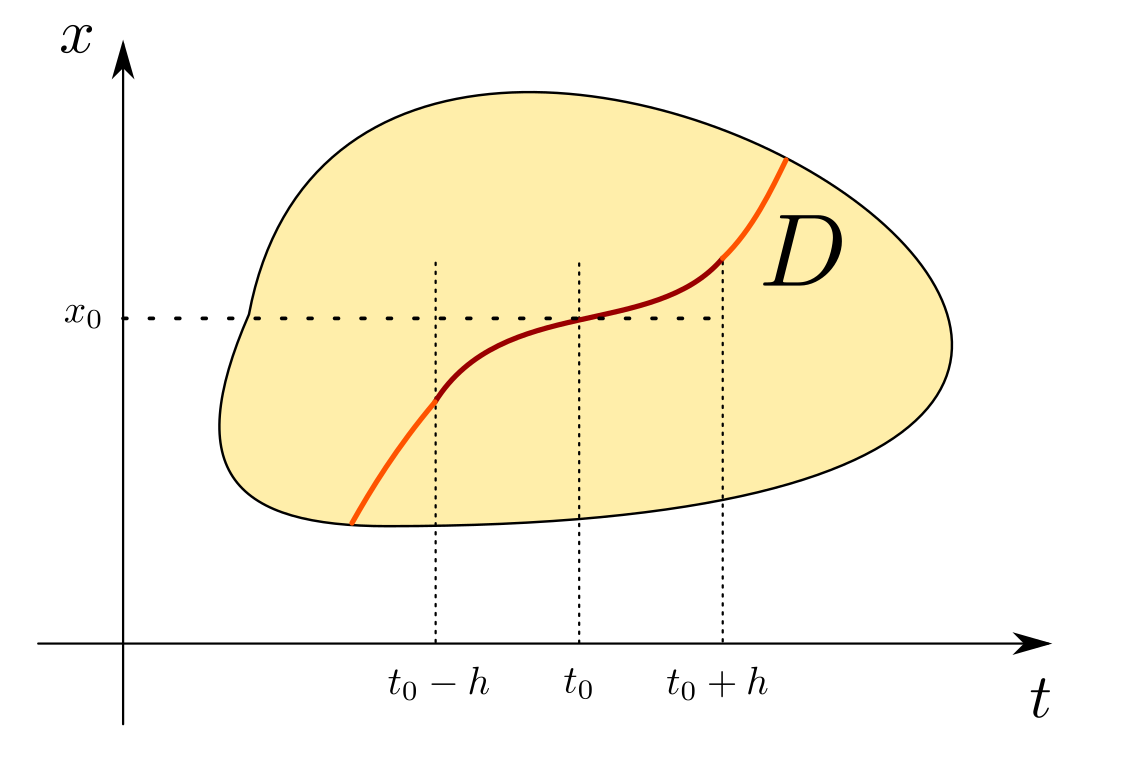
\includegraphics[scale=0.27]{assets/lectures-d0fd0868.png} \end{center}
    Тоді $\exists t^{-} $та  $t^{+} :  t^{-} < t < t^{+}$ такі, що розв'язок задачі Коші з початковою умовою існує на проміжку $ (t^{-}, t^{+})$, причому точки $ (t^-, \overline{x} (t^-)), (t^+, \overline{x} (t^+))$ належать межі області $D$.
\end{boxteo}
\subsection{Основні поняття теорії стійкості.}
Розглянемо систему диф. рівнянь $\overline{x}'(t) = \overline{f} (t, \overline{x})$:
$$f \in   \mathbb{C}(D)\qquad D = [a, +\infty ]  \times G\qquad G \in \mathbb{R}^{n} \qquad  \forall (t_0, \overline{x}^0) \in D  \exists! \text{ розв. З.К. } $$

\bd Розв'язок системи (1) називається стійким за Ляпуновим, якщо:\\
1) $\overline{x} = \overline{\varphi } (t)  \quad \exists$ на $[a, +\infty]$.\\
2) $\forall \varepsilon > 0 \quad \forall t_0 \geq a \quad \exists \delta > 0$, таке, що $ \left|\left| \overline{x}(t_0) - \overline{\varphi}(t_0) \right|\right| < \delta $ справедливо, що $ \left| \left|
\overline{x} (t) - \overline{\varphi} (t)
  \right|  \right|  < \delta  \quad \forall t \geq t_0$.
\ed

\bd
Розв'язок $ \overline{x} = \varphi(t) $ називається асимптотично стійким за Ляпуновим, якщо:
1. $ \overline{x} = \overline{\varphi} (t)$ - стійкий.\\
2. $\forall t_0 \geq a \quad \exists \delta > 0 \quad \forall \overline{x} (t) $ такого, що $ \left|
\left|  \overline{x} (t_0) - \overline{\varphi} (t_0) \right|
 \right| $ справедливо, що: \\ $  \left|
 \left|  \overline{x} (t) - \overline{\varphi} (t) \right|
  \right| \to 0   $ при $ t \to + \infty$
\ed

\def\vx{\overline{x}}
\def\vphi{\overline{\varphi}}
\def\vf{\overline{f}}

\bd
Роз'язок називається \textbf{нестійким}, якщо він не є стійким.
\ed

\subsection{Прилади дослідження на стійкість за означенням.}

\begin{example}
    Дослідити на стійкість розв'язок З.К.:
$$
\begin{cases}
    x = 1 \\
    x(0) = 0
\end{cases}
$$
1. Знайдемо розв'язок заданої З.К.: $x = 1 \Rightarrow x = t + C$ - заг. розв.\\
Підставимо: $ 0 = 0 + C \Longrightarrow C = 0 \Longrightarrow $ \fbox{ $ \varphi(t) = t $} - будемо досліджувати.
Зазначений розв'язок не має вертикальних асимптот та існує на всьому $\mathbb{R}$.
2. Знайдемо розв'язок довільної З.К. $x(t_0) = x_0$.
$$
x_0 = t_0 + C \Rightarrow C = x_0 - t_0 \Rightarrow x(t) = t + x_0 - t_0
$$
3. Нехай $  \left| x(t_0) - \varphi(t_0) \right|  =  \left| x_0 - t_0 \right| < \delta  $ ;\\
Тоді $ \left| x (t) - \varphi (t) \right|  = \left|  x_0 - t_0 \right| < \varepsilon = \delta $.\\
Таким чином, розв'язок є стійким, але не є асимптотично стійким.

\end{example}

\begin{example}
    Дослідити на стійкість розв'язок З.К.:
    $$
    \begin{cases}
        \dot{x} = 1 + t - x \\
        x(0) = 0
    \end{cases}
    $$
    1. Знайдемо розв'язок даної задачі Коші:
    $$
    \dot{x} = - x + 1 + t = \left| \text{ методом Бернуллі } \right| = t + Ae^{-t}
    $$
    Знайшли загальний розв'язок. Підставимо умову із з. К.: $ A = 0 \Rightarrow \fbox {$\varphi(t) = t$ }$\\
    2. Знайдемо розв'язок довільної З.К.:
    $$
    x(t_0) = x_0 \qquad x_0 = t_0 + Ae^{-t_0} \qquad A = (x_0 - t_0) e^{t_0}
    $$
    $$
    x(t) = t + (x_0 - t_0) e^{t_0 - t} - \text{ загальний розв'язок з. К.}
    $$

    3. Нехай $ \left|  x(t_0) - \varphi(t_0)  \right| = \left| x_0 - t_0 \right|  < \delta $. Розглядаємо: $ \forall t \geq t_0 :$
    $$
    \left| x(t) - \varphi(t) \right| = \left| t + (x_0 - t_0) \cdot e^{ t_0 - t} - t \right| =
     \left| x_0 - t_0 \right|< \delta  \to 0  \quad (t \to + \infty)
    $$
    Отримали, що знайдений розв'язок є асимптотично стійким.
\end{example}
Перейдемо знов до систем диф. рівнянь: $ \vx' = \vf (t, \vx)  \quad (1)$.\\
$\vx = \vphi (t)$ - розв'язок, який ми маємо дослідити на стійкість.\\
Заміна $ \overline{z} (t) = \vx (t)  - \vphi (y) $. Отримаємо систему:
$$ \overline{z}' + \overline{\varphi}'  = \overline{f} (t, \overline{z}+ \overline{\varphi})(t)$$
$$
\overline{f}' (t) = \overline{f} (t, \overline{\varphi})  \Longrightarrow \fbox{ $ \overline{z} ' = \overline{\varphi} (t, \overline{z} + \overline{\varphi} (t)) - \overline{f} ( t, \varphi(t)) $}
$$

Sample



\end{document}
